\documentclass[tikz,border=2pt]{standalone}
\usepackage{tikz}
\usetikzlibrary{backgrounds}
\begin{document}
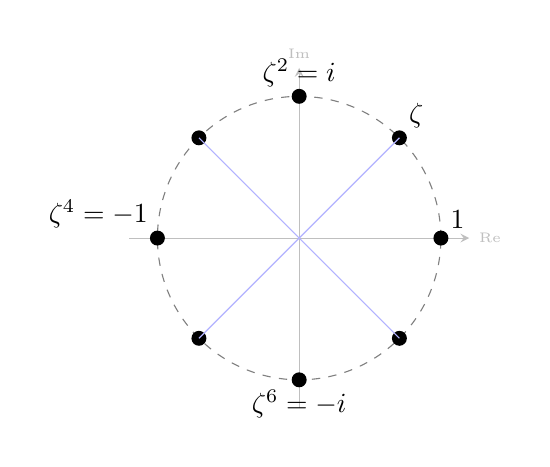
\begin{tikzpicture}[scale=1.8, background rectangle/.style={fill=white}, show background rectangle]    \def\R{1}
    \draw[gray, thin, dashed] (0,0) circle (\R);
    \draw[->, >=stealth, gray!50] (-1.2,0) -- (1.2,0) node[right] {\tiny Re};
    \draw[->, >=stealth, gray!50] (0,-1.2) -- (0,1.2) node[above] {\tiny Im};
    
    \foreach \k in {0,...,7} {
        \coordinate (P\k) at ({\k*360/8}:\R);
        \fill (P\k) circle (1.5pt);
    }
    
    \node[above right] at (P0) {$1$};
    \node[above right] at (P1) {$\zeta$};
    \node[above] at (P2) {$\zeta^2 = i$};
    \node[above left] at (P4) {$\zeta^4 = -1$};
    \node[below] at (P6) {$\zeta^6 = -i$};
    
    \draw[blue!30, thin] (P1) -- (P5);
    \draw[blue!30, thin] (P3) -- (P7);
\end{tikzpicture}
\end{document}